\documentclass[tikz]{standalone}
\usepackage{fourier}
\usetikzlibrary{arrows.meta}
\usetikzlibrary{calc}
\tikzset{>=latex}
\definecolor{bookblue}{RGB}{0,173,239}
\definecolor{bookpink}{RGB}{236,0,140}
\definecolor{bookgreen}{RGB}{50,200,0}
\definecolor{bookbluearea}{RGB}{204,239,252}
\tikzstyle{blueline}=[draw=bookblue,line width=0.2mm]
\tikzstyle{pinkline}=[draw=bookpink,line width=0.2mm]
\tikzstyle{greenline}=[draw=bookgreen,line width=0.2mm]
\tikzstyle{blackline}=[draw=black,line width=0.2mm]
\tikzstyle{bluearea}=[fill=bookbluearea]

\begin{document}
  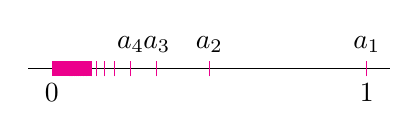
\begin{tikzpicture}
  	\xdef\qtd{4}
    \draw (-.3,0) -- (\qtd.3,0);
		\fill [bookpink] (0,-0.1) rectangle (0.5,.1);
    \node at (0,-0.3) {0};
    \node at (\qtd,-0.3) {1};
    \foreach \x in {1,...,18}{
      \draw [bookpink](\qtd/\x,-0.1) -- (\qtd/\x,0.1);
      
    }
  	\foreach \x in {1,...,4}{
  		\node at (\qtd/\x,0.3) {$a_\x$};
  	}
    
  \end{tikzpicture}
\end{document}